\chapter{High Intensity Studies}
\label{sec:ch6}

\section{Global RDTs and Intensity-Dependent Effects}
\cite{mionrr}
\section{Space Charge Tune Shift}

\begin{equation}
    \Delta \nu_{sc}=\frac{-3 N r_0 R S}{4 \sigma_z M \beta \gamma ^2 \varepsilon_{N,95\%}}    
\end{equation}

\section{Measurement of Tune Shift}

% \newpage
% \begin{figure}[H]
%     \centering
%     \includegraphics[height=\textheight,keepaspectratio]{chapter6/scts_measure.png}
%     \caption{Tune spread.}
%     \label{fig:dynamictunespread}
% \end{figure}
% \newpage

\begin{figure}[H]
    \centering
    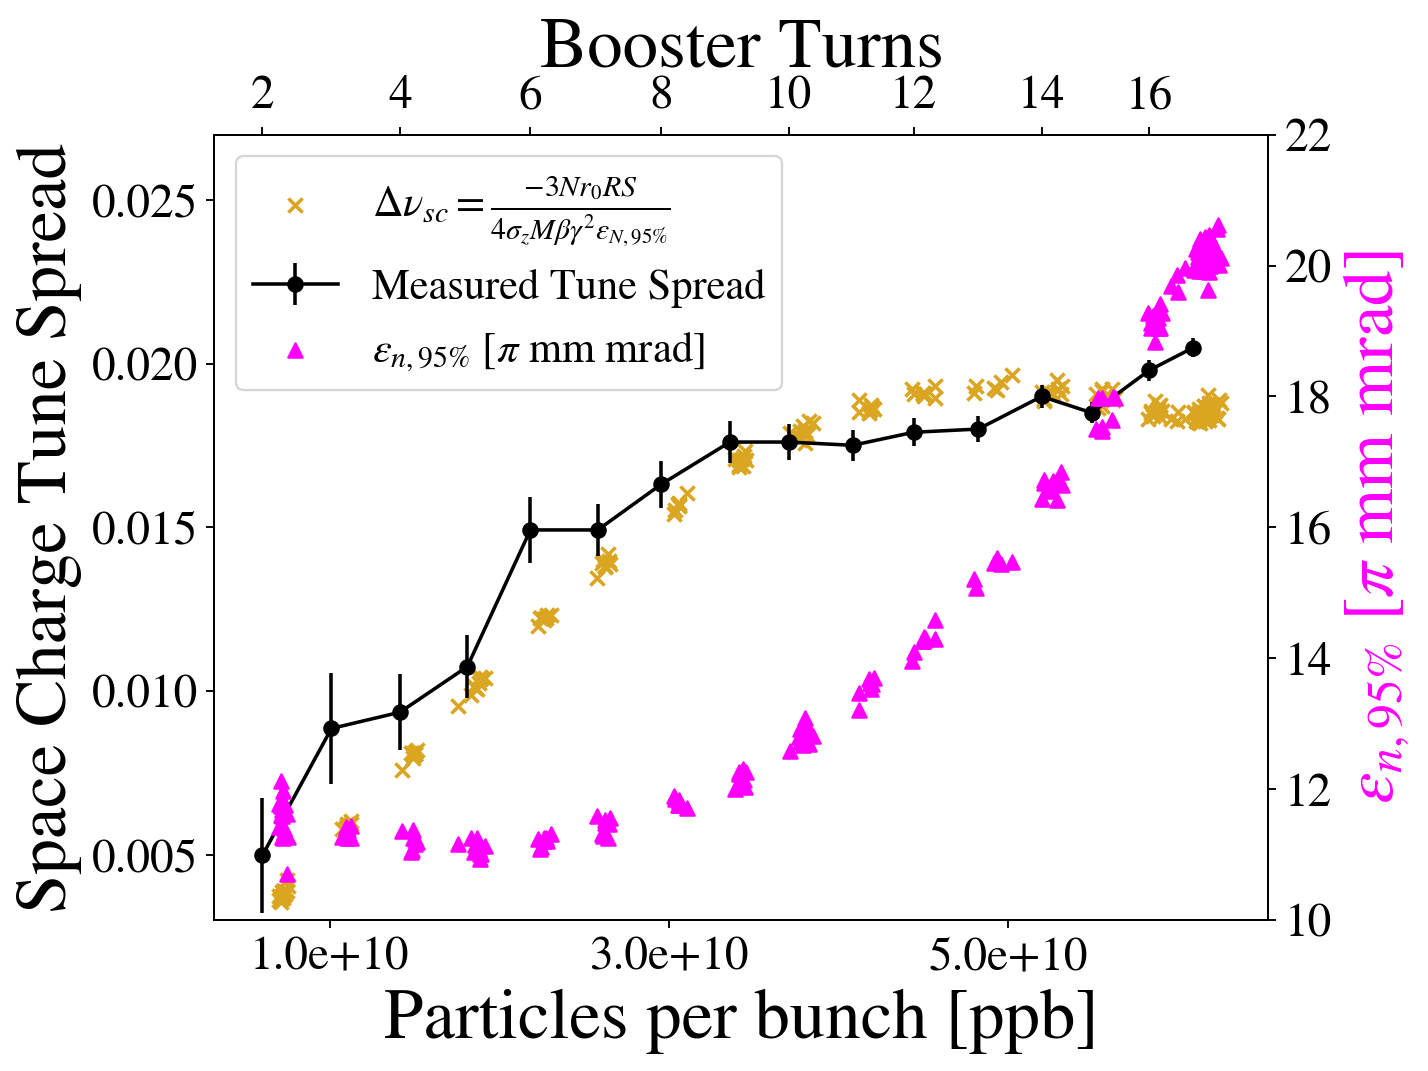
\includegraphics[width=\columnwidth]{chapter6/tune_spread.png}
    \caption{Measurement of tune spread.}
    \label{fig:tunespread}
\end{figure}

\section{Static Tune Scans at Different Intensities}
